\documentclass[
version=last,toc=bib,toc=graduated,toc=index,toc=listof,9pt,openany]{scrbook}
%\pdfminorversion=4
\usepackage{polyglossia}
\setdefaultlanguage{english}

\setmainfont{Source Sans Pro}
\setsansfont{Source Sans Pro}

\usepackage{ifmtarg}
\usepackage{ifthen}
\usepackage{etoolbox} % \ifstrempty

\usepackage{geometry}
\geometry{%a6paper
paperwidth=125mm, paperheight=168mm, 
portrait,
top=22mm,
inner=22mm,
outer=20mm,
bottom=25mm,
headsep=3mm,
footskip=12mm
}

% math symbols
\usepackage{amssymb}

\usepackage{ragged2e} % nicer typesetting (hyphenation) for non raggedright and raggedleft
\usepackage{lscape}
\setlength{\parskip}{0pt}

\usepackage{relsize}

\clubpenalty=10000
\widowpenalty=10000 
\displaywidowpenalty=10000

\usepackage[]{microtype}

\usepackage{graphicx} % graphics

% search path for images
\graphicspath{{images-print/}{icons/}{extra-pages/}{wallpaper/}}
\usepackage{wrapfig}  % sponsor logos wrapped with text

\usepackage{tabu}
\usepackage[table,cymk]{xcolor}
\usepackage{colortbl}

% embed PDF pages
% pdfpages must not be loaded before colortbl!
\usepackage{pdfpages}
% TikZ must not be loaded before colortbl
\usepackage{tikz}

\usepackage{multirow}
%\usepackage{booktabs}

\usepackage{array}

% dashed lines in tables
\usepackage{arydshln}
\ADLdrawingmode{1}

% multiple text columns (list of thanks)
\usepackage{multicol}

\usepackage{refcount} % calculation of the page where the map is located

% page background
\usepackage[manualmark]{scrlayer-scrpage}
\pagestyle{scrplain}

\newcommand{\acro}[1]{{\textsmaller{#1}}} % macro for abbreviations with more than one capitalised letter


% title/metadata
\title{State of the Map 2019}
\subtitle{Programme}
\author{OpenStreetMap Foundation}
\date{\today}

\clearscrheadings

% page numbers
\cfoot[\begin{small}\pagemark\end{small}]{\begin{small}\pagemark\end{small}}
\ofoot[]{}
\ifoot[]{}
\pagestyle{scrplain}

\linespread{1.15}

% include our custom macros
% command for a new time slot
\newcommand{\talkTime}{9:99}
\newcommand{\newTimeslot}[1]{\newpage\renewcommand{\talkTime}{#1}}

% new time slot but without a pagebreak
\newcommand{\newSmallTimeslot}[1]{\renewcommand{\talkTime}{#1}}

% initialise \conferenceDay
\newcommand{\conferenceDay}{Noday}


% define default page style (cutting marks with page number)
\DeclareNewLayer[background, oddorevenpage, width=125mm,%
height=169mm, contents={%
  
\includegraphics{wallpaper/crop-marks.pdf}%
}]{cropmarksevery}
\newpairofpagestyles[scrheadings]{cropmarksstyle}{}
\AddLayersAtBeginOfPageStyle{cropmarksstyle}{cropmarksevery}

% page style for title pages
\DeclareNewLayer[background, oddorevenpage, width=125mm,%
height=169mm, contents={%
  
\includegraphics{wallpaper/front-cover-with-crop-marks.pdf}%
}]{titlelayer}
\newpairofpagestyles[]{titlestyle}{}
\AddLayersAtBeginOfPageStyle{titlestyle}{titlelayer}

% define alias commands for all three days
\def\saturday{Saturday}
\def\sunday{Sunday}
\def\monday{Monday}

% define Saturday page style
\DeclareNewLayer[background, oddpage,  width=125mm,%
height=169mm, contents={%
  
\includegraphics{wallpaper/saturday-odd.pdf}%
}]{saturdayodd}
\DeclareNewLayer[background, evenpage,  width=125mm,%
height=169mm, contents={%
  
\includegraphics{wallpaper/saturday-even.pdf}%
}]{saturdayeven}
\DeclareNewLayer[background, oddpage,  width=125mm,%
height=169mm, contents={%
  
\includegraphics{wallpaper/saturday-odd-rotated.pdf}%
}]{saturdayoddrotated}
\newpairofpagestyles[scrheadings]{saturday-table}{}
\AddLayersAtBeginOfPageStyle{saturday-table}{saturdayeven}
\AddLayersAtBeginOfPageStyle{saturday-table}{saturdayoddrotated}
\newpairofpagestyles[scrheadings]{saturday}{}
\AddLayersAtBeginOfPageStyle{saturday}{saturdayeven}
\AddLayersAtBeginOfPageStyle{saturday}{saturdayodd}

% define Sunday page style
\DeclareNewLayer[background, oddpage,  width=125mm,%
height=169mm, contents={%
  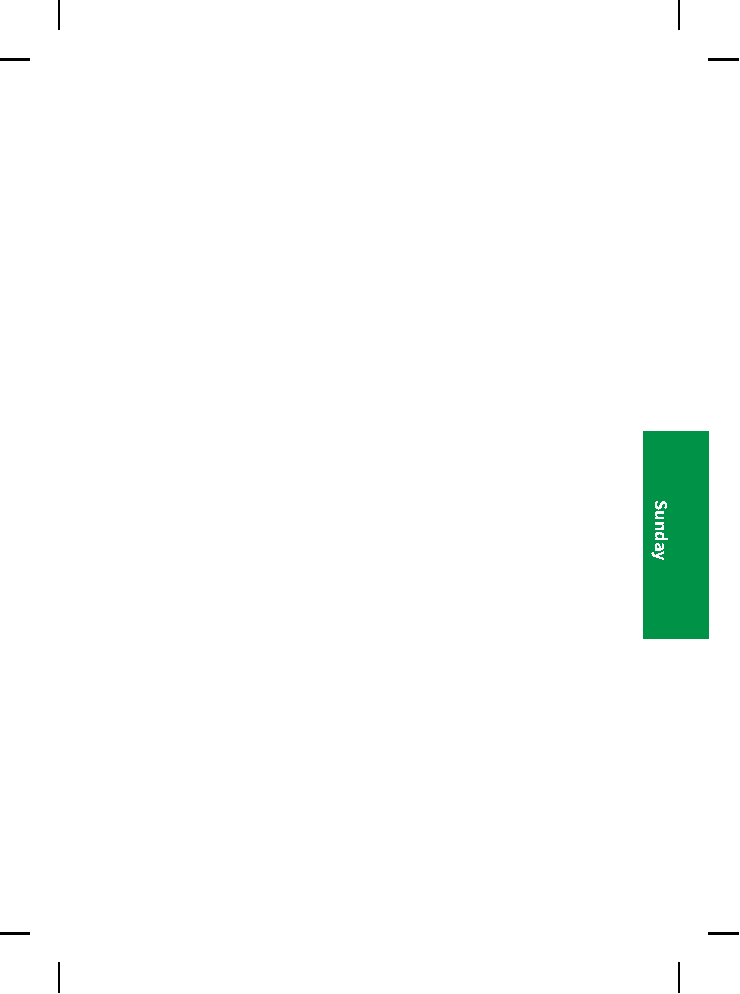
\includegraphics{wallpaper/sunday-odd.pdf}%
}]{sundayodd}
\DeclareNewLayer[background, evenpage,  width=125mm,%
height=169mm, contents={%
  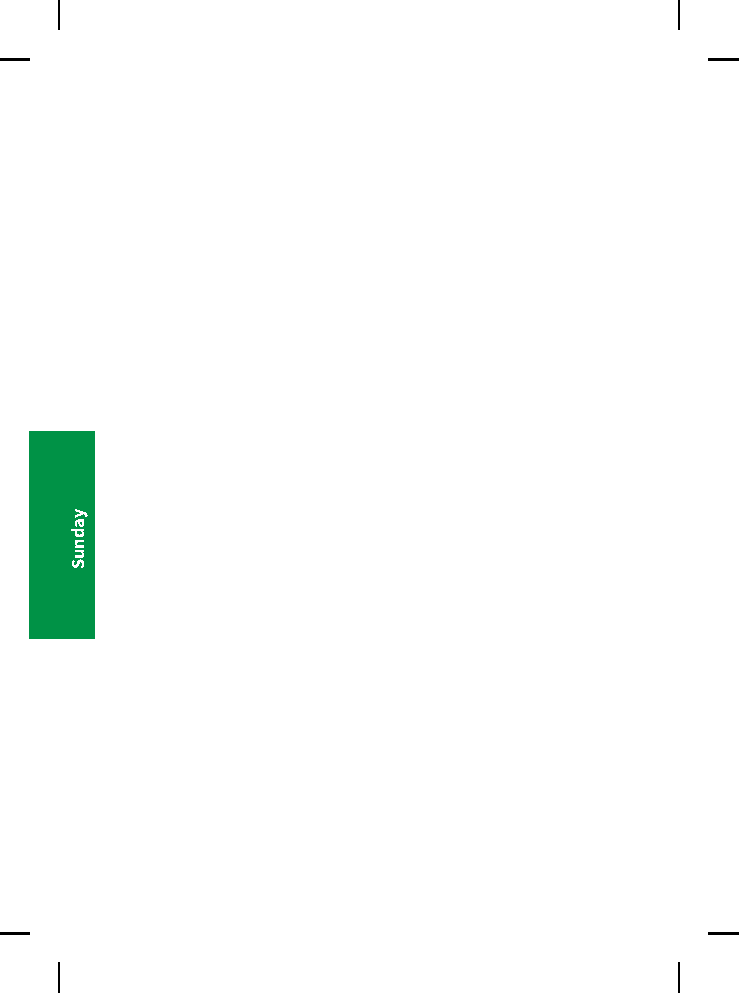
\includegraphics{wallpaper/sunday-even.pdf}%
}]{sundayeven}
\DeclareNewLayer[background, oddpage,  width=125mm,%
height=169mm, contents={%
  
\includegraphics{wallpaper/sunday-odd-rotated.pdf}%
}]{sundayoddrotated}
\newpairofpagestyles[scrheadings]{sunday-table}{}
\AddLayersAtBeginOfPageStyle{sunday-table}{sundayeven}
\AddLayersAtBeginOfPageStyle{sunday-table}{sundayoddrotated}
\newpairofpagestyles[scrheadings]{sunday}{}
\AddLayersAtBeginOfPageStyle{sunday}{sundayeven}
\AddLayersAtBeginOfPageStyle{sunday}{sundayodd}

% define Monday page style
\DeclareNewLayer[background, oddpage,  width=125mm,%
height=169mm, contents={%
  
\includegraphics{wallpaper/monday-odd.pdf}%
}]{mondayodd}
\DeclareNewLayer[background, evenpage,  width=125mm,%
height=169mm, contents={%
  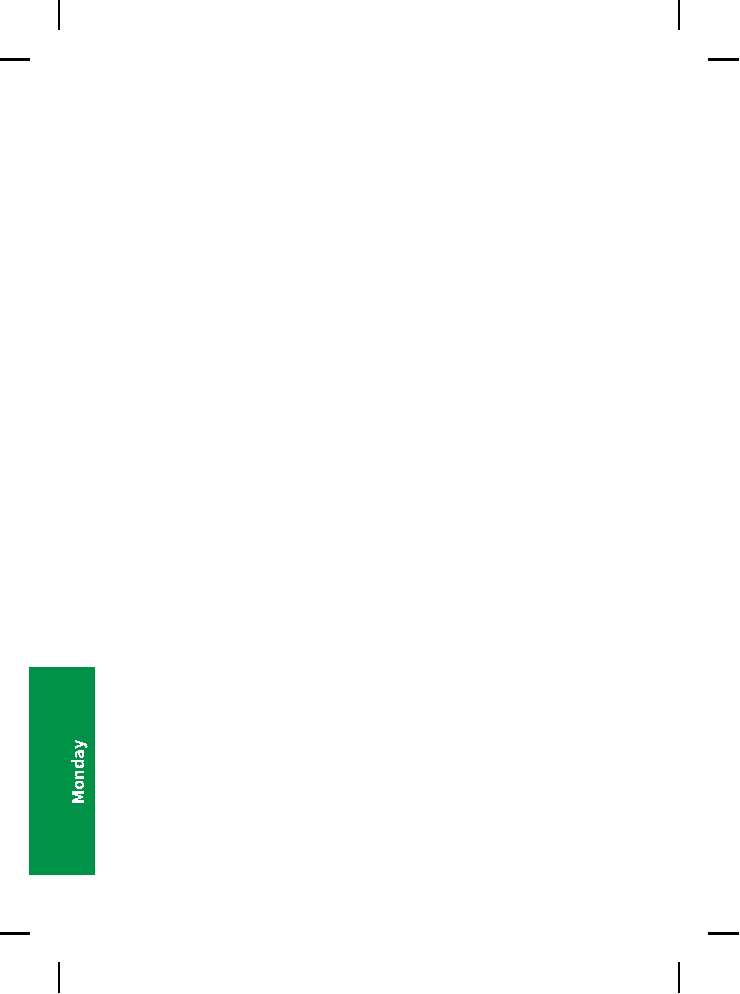
\includegraphics{wallpaper/monday-even.pdf}%
}]{mondayeven}
\DeclareNewLayer[background, oddpage,  width=125mm,%
height=169mm, contents={%
  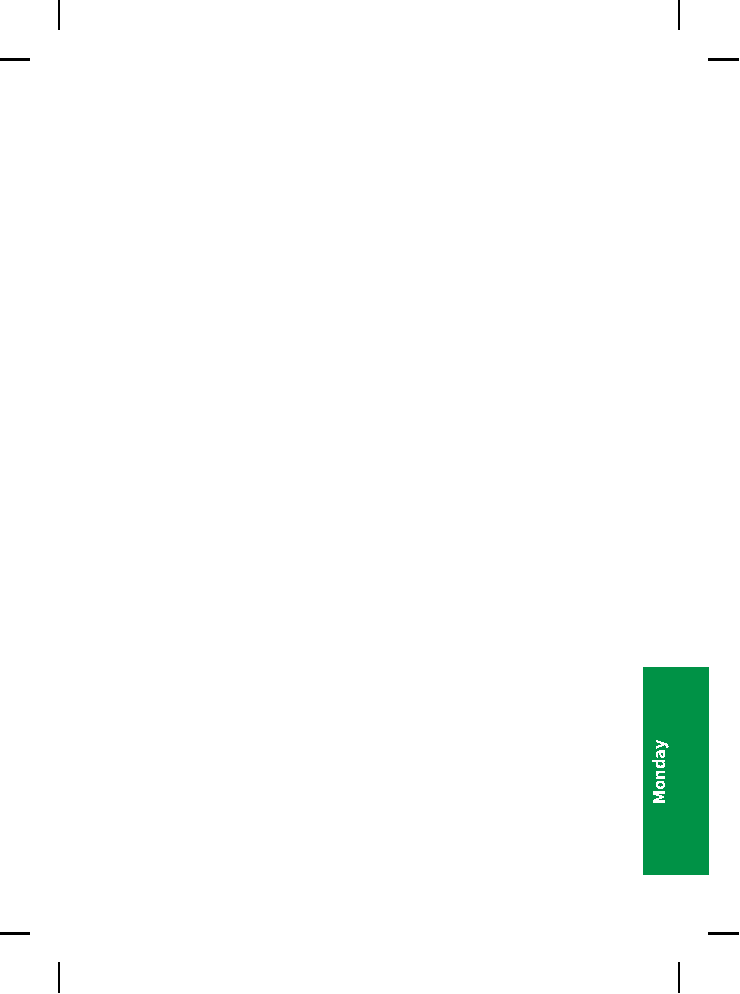
\includegraphics{wallpaper/monday-odd-rotated.pdf}%
}]{mondayoddrotated}
\newpairofpagestyles[scrheadings]{monday-table}{}
\AddLayersAtBeginOfPageStyle{monday-table}{mondayeven}
\AddLayersAtBeginOfPageStyle{monday-table}{mondayoddrotated}
\newpairofpagestyles[scrheadings]{monday}{}
\AddLayersAtBeginOfPageStyle{monday}{mondayeven}
\AddLayersAtBeginOfPageStyle{monday}{mondayodd}

% \setpagebackground selects the page style to be used depending on the current day. Each day has
% its own page style.
\newcommand{\setPageBackground}{ %
  \ifthenelse{\equal{\conferenceDay}{\saturday}}{%
    \pagestyle{saturday}
  }{}
  \ifthenelse{\equal{\conferenceDay}{\sunday}}{%
    \pagestyle{sunday}
  }{}
  \ifthenelse{\equal{\conferenceDay}{\monday}}{%
    \pagestyle{monday}
  }{}
}


% additional column type for tables
\newcolumntype{Y}[1]{>{\RaggedRight\arraybackslash}p{#1}}

%% length of the title boxes
\newlength{\titleboxwidth}
\advance\titleboxwidth by -6pt

\newlength{\roomWidth}
\newlength{\timeWidth}
\newlength{\roomTimeWidth}
\newlength{\titleWidth}
\newcommand{\tmpRoomTimeWidth}{}
\newcommand{\tmpTitleWidth}{}

\newcommand{\setAbstract}[6]{%
  % 1. speaker
  % 2. title
  % 3. subtitle
  % 4. abstract (Text)
  % 5. colour
  % 6. room
  \setPageBackground%
  \calculateRoomTimeAndTitleWidth{#1}{#6}%
  \noindent\fcolorbox{white}{#5}{%
    \parbox{\titleboxwidth}{%
      \isSpeakerEmpty{#1}{#2}{#6}%
      \isSubtitleEmpty{#3}%
    }%
  }%
  %
  \isAbstractEmpty{#4}%
  \vspace{0.5em}% space to the next talk even if there is no abstract
}

% Calculate width of title and room/time field
% Arguments: speaker, room
\makeatletter
  \newcommand{\calculateRoomTimeAndTitleWidth}[2]{%
    \@ifmtarg{#1}{% speaker is empty
      \settowidth{\roomWidth}{#2, \talkTime}%
    }{% speaker is not empty
      \settowidth{\roomWidth}{#2}%
    }%
    \settowidth{\timeWidth}{\talkTime}%
    \directlua{require("lua/titleWidth")}%
    \setlength{\titleboxwidth}{\directlua{getTitleBoxWidth()}}%
    \renewcommand{\tmpRoomTimeWidth}{\directlua{getTimeRoomWidth()}}%
    \setlength{\roomTimeWidth}{\tmpRoomTimeWidth}%
    \renewcommand{\tmpTitleWidth}{\directlua{getTitleWidth()}}%
    \setlength{\titleWidth}{\tmpTitleWidth}%
  }%
\makeatother

% Lay out the subtitle
% has to be a separate function and has to be surrounded by \makeatletter for technical reasons
\makeatletter
  \newcommand{\isSubtitleEmpty}[1]{%
    \@ifnotmtarg{#1}{%
      \par
      \RaggedRight
      \vspace{0.5\baselineskip}
      \noindent%
      \bfseries%
      #1%
    }
  }
\makeatother

% lay out the speaker if there is any
% We assume that there is only a subtitle if the talk has a speaker.
\makeatletter
  \newcommand{\isSpeakerEmpty}[3]{%
    % Arguments:
    % 1. speaker
    % 2. title
    % 3. room
    \@ifmtarg{#1}{%
      \begin{minipage}[t][][t]{\titleWidth}
        \RaggedRight
        \noindent%
        {\large \sectfont #2}%
      \end{minipage}%
      \hfill
      \begin{minipage}[t][][t]{\roomTimeWidth}
        \RaggedLeft%
        \noindent #3, \talkTime%
      \end{minipage}%
    }%
    {%
      \begin{minipage}[t][][t]{\titleWidth}
        \RaggedRight
        \emph{#1} % speaker
        \par%
        \vspace{0.3\baselineskip}
        \noindent%
        {\large \sectfont #2}%
      \end{minipage}%
      \hfill
      \begin{minipage}[t][][t]{\roomTimeWidth}
        \RaggedLeft
        \talkTime%
        \par%
        \noindent #3% room
      \end{minipage}%
    }%
  }
\makeatother

% Lay out the abstract if there is any
% has to be a separate function and has to be surrounded by \makeatletter for technical reasons
\makeatletter
\newcommand{\isAbstractEmpty}[1]{%
  \ifstrempty{#1}{%
    \vspace{1.5em}%
  }{%
    \vspace{0.5em}\newline%
    #1 \par% % abstract
    \vspace{1.5em}% space to the next talk even if there is an abstract
  }%
}
\makeatother

% define colours
\definecolor{GHS}{cmyk}{0.16 0 .05 0}
\definecolor{HSO}{cmyk}{0.02 0 0.12 0.11}
%\definecolor{academic}{cmyk}{0 0.02 0.23 0}
\definecolor{academic}{cmyk}{0.35 0 0.33 0.16}
\definecolor{HSW}{cmyk}{0.35 0 0.33 0.16}
\definecolor{KHS}{cmyk}{0 .24 0.29 .04}
\definecolor{Mathematikon C}{cmyk}{.16 0 0.35 0}
\definecolor{ochsenblutrot}{cmyk}{0 0.72 0.65 0.65}

% session at GHS
\newcommand{\abstractGHS}[4]%
{%
  \setAbstract{#1}{#2}{#3}{#4}{GHS}{GHS}
}

% abstract at HSO
\newcommand{\abstractHSO}[4]%
{%
  \setAbstract{#1}{#2}{#3}{#4}{HSO}{HSO}
}

% abstract for academic talks
\newcommand{\abstractAcademic}[4]%
{%
  \setAbstract{#1}{#2}{#3}{#4}{academic}{HSW}
}

% abstract at HSW
\newcommand{\abstractHSW}[4]%
{%
  \setAbstract{#1}{#2}{#3}{#4}{HSW}{HSW}
}

% abstract at KHS
\newcommand{\abstractKHS}[4]%
{%
  \setAbstract{#1}{#2}{#3}{#4}{KHS}{KHS}
}

% abstract at Mathematikon C
\newcommand{\abstractMathematikonC}[4]%
{%
  \setAbstract{#1}{#2}{#3}{#4}{Mathematikon C}{Mathematikon C}
}

% abstract at a different location
\newcommand{\abstractOther}[5]%
{%
  \setAbstract{#1}{#2}{#3}{#4}{commongray}{#5}
}

% infobox for workshops (they don't have an abstract in the booklet)
\newcommand{\workshopbox}[3]{%
  % 1. titel
  % 2. speaker
  % 3. Room
  \setlength\tabcolsep{0pt}
  \noindent\fcolorbox{white}{dezentrot}{%
    \parbox{\titleboxwidth}{%
      \noindent%
      \begin{tabu}{X[5L]r}
        \emph{#2} % Sprecher
        &
        \talkTime
        \tabularnewline
        {\noindent\large \bfseries #1}% % title
        &
        #3
        \tabularnewline
      \end{tabu}
    }
  }
  \setlength\tabcolsep{6pt} % set column padding back to default
}

% too long
\newcommand{\tooLong}{Dieser Text ist viel zu lang. Dieser Text ist viel zu lang. Dieser Text ist viel zu lang. Dieser Text ist viel zu lang. Dieser Text ist viel zu lang. Dieser Text ist viel zu lang. Dieser Text ist viel zu lang. Dieser Text ist viel zu lang. Dieser Text ist viel zu lang. Dieser Text ist viel zu lang. Dieser Text ist viel zu lang. Dieser Text ist viel zu lang. Dieser Text ist viel zu lang. Dieser Text ist viel zu lang. }

\newlength{\fboxwidth}

\def\workshopsSection{workshopsSection}
\def\abstractsSection{abstractsSection}

% boxes for text-only advertisement texts by our sponsors
\newcommand{\sponsorBox}[4]{%
  \setlength{\fboxwidth}{\textwidth}
  \advance\fboxwidth by -7.0pt
  \abstractSponsorbox{#1}{#2}{#3}{#4}{\workshopsSection}%
}

\newcommand{\sponsorBoxA}[4]{%
  \setlength{\fboxwidth}{\textwidth}
  \advance\fboxwidth by -10.0pt
  \abstractSponsorbox{#1}{#2}{#3}{#4}{\abstractsSection}%
}

%% store \parindent in separate variable because it is resetted to 0 in parboxes
\newlength{\saveparindent}
\setlength{\saveparindent}{\parindent}

%% box for advertisment by a sponsor
%% 1. logo
%% 2. width of the logo
%% 3. number of required lines of the logo (due to usage of wrapfigure)
%% 4. text
%% 5. Umfeld (\workshopsSection oder \abstractsSection}
\makeatletter
  \newcommand{\abstractSponsorbox}[5]{%
    \setlength{\fboxsep}{4.5pt}%
    \noindent%
    \ifthenelse{\equal{#5}{\workshopsSection}}{%
      \hspace{2.65pt}%
    }{%
      \hspace{-1pt}%
    }%
    \fcolorbox{gray}{white}{%
      \parbox{\fboxwidth}{
        \setlength{\parindent}{\saveparindent}%
        \@ifmtarg{#1}{}{%
          \begin{wrapfigure}[#3]{r}[0pt]{#2}
            \centering\vspace{-1\baselineskip}
            \includegraphics[width=#2]{#1}
          \end{wrapfigure}
        }

        \noindent #4
      }%
    }
    \setlength{\fboxsep}{3pt}
  }
  \setlength{\fboxsep}{3pt}
\makeatother

% definition of column types for the schedule tables
\newcolumntype{Z}[1]{>{\RaggedRight\arraybackslash}p{#1}}%
\newcolumntype{C}[1]{>{\Centering\arraybackslash}p{#1}}%

% common implementation of typesetting of a session in the tables
\newcommand{\talkInternal}[2]{%
  \textbf{#1}
  \ifthenelse{\equal{#2}{}}{}{%
    \newline\emph{#2}%
  }
}

% macro to typeset a talk in the schedule tables spanning over more than one row:
% usage: \longTalk{rowcount}{title}{speaker}
\newcommand{\longTalk}[3]{%
  &
  \multirow{#1}{\linewidth}{%
    \parbox{\linewidth}{
      %HACK Inserting a \vspace here is a dirty hack but it works.
      \vspace{0.45\baselineskip}
      \talkInternal{#2}{#3}%
    }
  }%
}%

% macro to typeset a talk in the schedule tables:
% usage: \talk{title}{speaker}
\newcommand{\talk}[2]{%
  &
  \talkInternal{#1}{#2}%
}%


% macro to typeset a talk in the schedule tables spanning over more than one column:
% usage: \multiColTalk{columns}{columnSpecs}{title}{speaker}
\newcommand{\multiColTalk}[4]{%
  &
  \multicolumn{#1}{#2}{\talkInternal{#3}{#4}}%
}%

\newcommand{\workshop}[3]%
{%
  \workshopbox{#1}{#2}{#3}
}%

\newcommand{\otherevent}[1]%
{%
  & \textbf{#1}
}%

\newcommand{\audimaxEvent}[2]%
{%
  &
  \multicolumn{3}{c}{
    \textbf{#1} (Audimax) \par \emph{#2}
  }
}%

\newcommand{\coffeespace}{\vspace{0.4em}}
\newcommand{\workshopspace}{\vspace{0.5em}\\}

% define colors
\definecolor{commongray}{gray}{.9}
\definecolor{tableRuleGray}{gray}{.4}
\definecolor{textGray}{gray}{.45}

% macro for table rules
\newcommand{\programCRule}[1]{%
  \arrayrulecolor{tableRuleGray}%
  \cdashline{#1}[0.2mm/0.4mm]%
}
\newcommand{\programHRule}[1]{%
  \arrayrulecolor{tableRuleGray}%
  \cdashline{2-#1}[0.2mm/0.4mm]%
}

% macro for empty session slots
\newcommand{\bookableSpace}{
  &
  \emph{\textcolor{textGray}{bookable space}}%
}

% diamond symbol for shortened titles
\newcommand{\diamondSymbol}{%
  \textsuperscript{%
    \diamond%
  }%
}

% speaker affiliation
\newcommand{\speakerAffiliation}[1]{%
  (#1)%
}

% lightning talk (title and author)
\newcommand{\lightningTalk}[2]{%
  \item \emph{#2:} #1%
}

% macro for no-video icon
\newcommand{\noVideo}{%
  
\includegraphics[height=9pt]{novideo.pdf}%
}

% skip line to make right/left table columns align
\newcommand{\skipline}{%
  \vspace{0.365cm}
}

%% Ministerium für Verkehr advertisement (left)
%TODO get rid of their cropmarks, add ours
\DeclareNewLayer[background,%
  width=115mm,%
  height=158mm,%
  hoffset=5mm,%
  voffset=5mm,%
  contents={%
    %TODO correct size
    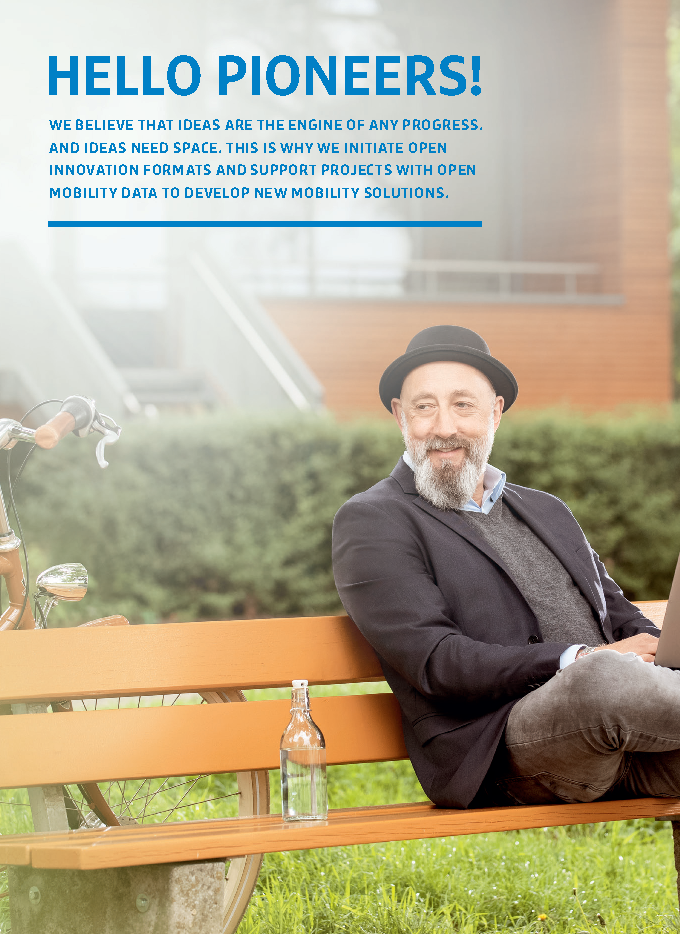
\includegraphics[pagebox=mediabox]{sponsors/ministerium-fuer-verkehr-left.pdf}%
  }%
]{mvleftadvertisement}
\newpairofpagestyles[]{sponsor-mvleft}{}
\AddLayersAtBeginOfPageStyle{sponsor-mvleft}{cropmarksplain}
\AddLayersAtBeginOfPageStyle{sponsor-mvleft}{mvleftadvertisement}

% Ministerium für Verkehr advertisement (right)
%TODO get rid of their cropmarks, add ours
\DeclareNewLayer[background,%
  width=115mm,%
  height=158mm,%
  hoffset=5mm,%
  voffset=5mm,%
  contents={%
    %TODO correct size
    
\includegraphics[pagebox=mediabox]{sponsors/ministerium-fuer-verkehr-right.pdf}%
  }%
]{mvrightadvertisement}
\newpairofpagestyles[]{sponsor-mvright}{}
\AddLayersAtBeginOfPageStyle{sponsor-mvright}{cropmarksplain}
\AddLayersAtBeginOfPageStyle{sponsor-mvright}{mvrightadvertisement}

% Geotab advertisement
\DeclareNewLayer[background,%
  width=125mm,%
  height=168mm,%
  hoffset=-0.4mm,%
  contents={%
    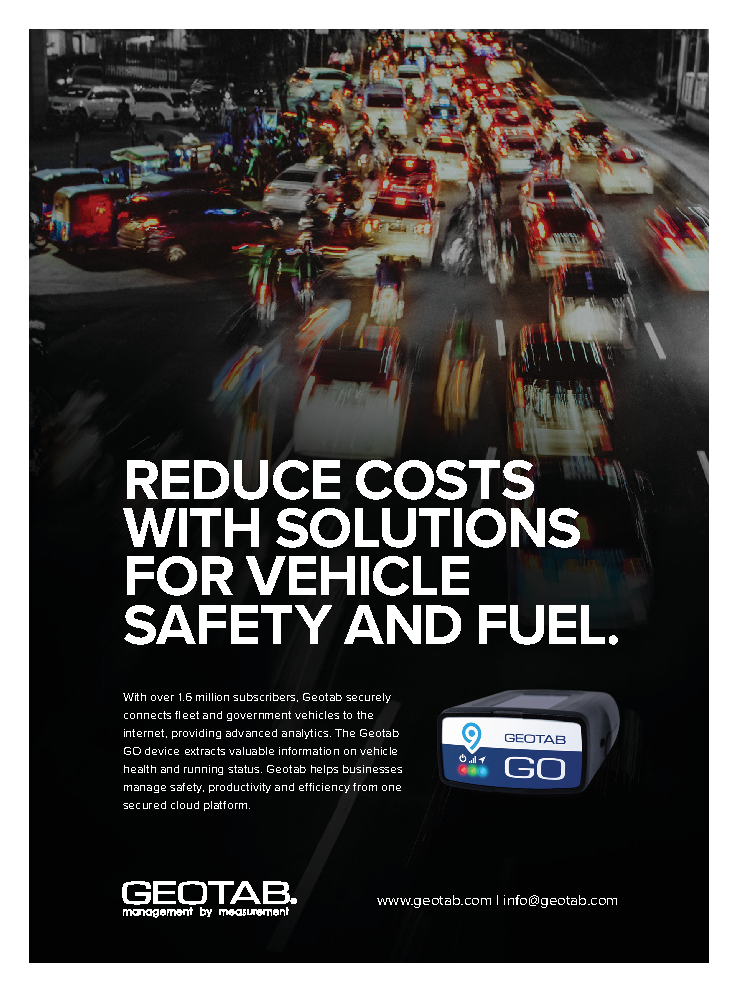
\includegraphics{sponsors/geotab.pdf}%
  }%
]{geotabadvertisement}
\newpairofpagestyles[]{sponsor-geotab}{}
\AddLayersAtBeginOfPageStyle{sponsor-geotab}{geotabadvertisement}
\AddLayersAtBeginOfPageStyle{sponsor-geotab}{cropmarksplain}

% Grab advertisement
\DeclareNewLayer[background,%
  width=125mm,%
  height=168mm,%
  hoffset=-0.4mm,%
  contents={%
    
\includegraphics{sponsors/grab.pdf}%
  }%
]{grabadvertisement}
\newpairofpagestyles[]{sponsor-grab}{}
\AddLayersAtBeginOfPageStyle{sponsor-grab}{grabadvertisement}
\AddLayersAtBeginOfPageStyle{sponsor-grab}{cropmarksplain}

% Mapbox advertisement
\DeclareNewLayer[background,%
  width=125mm,%
  height=168mm,%
  contents={%
    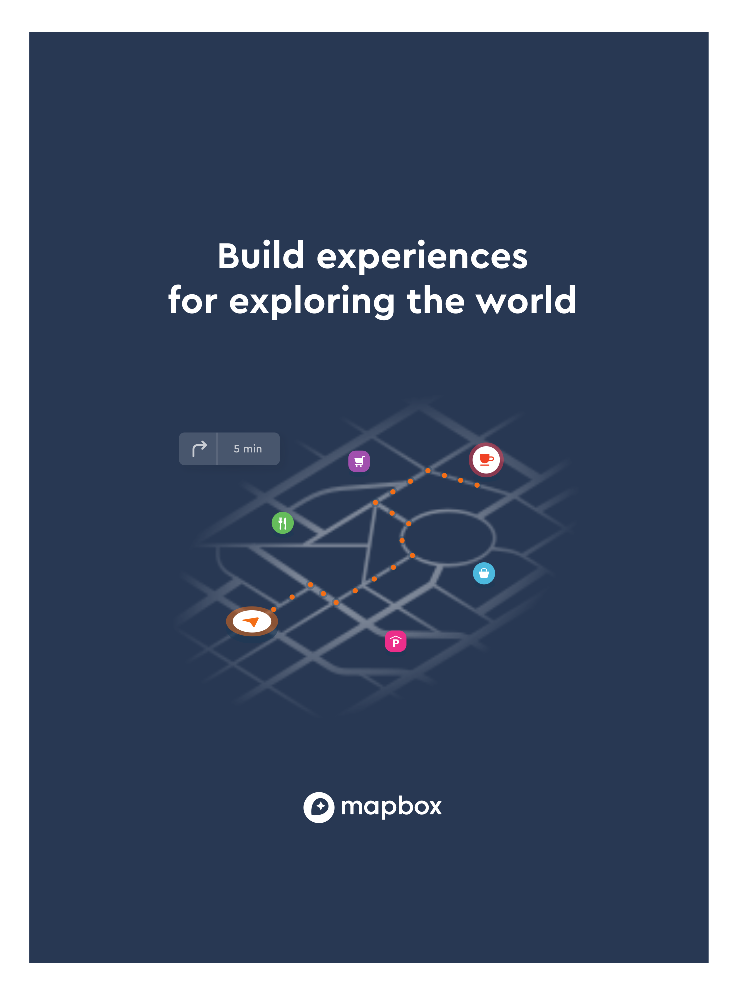
\includegraphics{sponsors/mapbox.pdf}%
  }%
]{mapboxadvertisement}
\newpairofpagestyles[]{sponsor-mapbox}{}
\AddLayersAtBeginOfPageStyle{sponsor-mapbox}{cropmarksplain}
\AddLayersAtBeginOfPageStyle{sponsor-mapbox}{mapboxadvertisement}

% Anyways advertisement
\DeclareNewLayer[background,%
  width=125mm,%
  height=168mm,%
  hoffset=-0.4mm,%
  contents={%
    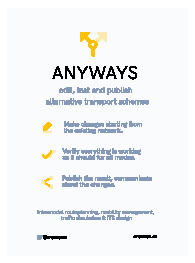
\includegraphics[width=125mm]{sponsors/anyways.pdf}%
  }%
]{anywaysadvertisement}
\newpairofpagestyles[]{sponsor-anyways}{}
\AddLayersAtBeginOfPageStyle{sponsor-anyways}{anywaysadvertisement}
\AddLayersAtBeginOfPageStyle{sponsor-anyways}{cropmarksplain}

% Telenav advertisement
\DeclareNewLayer[background,%
  width=125mm,%
  height=168mm,%
  hoffset=-0.4mm,%
  contents={%
    
\includegraphics[width=125mm]{sponsors/telenav.png}%
  }%
]{telenavadvertisement}
\newpairofpagestyles[]{sponsor-telenav}{}
\AddLayersAtBeginOfPageStyle{sponsor-telenav}{cropmarksplain}
\AddLayersAtBeginOfPageStyle{sponsor-telenav}{telenavadvertisement}

% OpenCage and Mapillary advertisement
\DeclareNewLayer[background,%
  width=115mm,%
  height=79mm,%
  hoffset=5mm,
  voffset=5mm,
  contents={%
    
\includegraphics[width=115mm, height=79mm]{sponsors/opencage.png}%
  }%
]{opencage}
\DeclareNewLayer[background,%
  width=115mm,%
  height=79mm,%
  hoffset=5mm,%
  voffset=84mm,%
  contents={%
    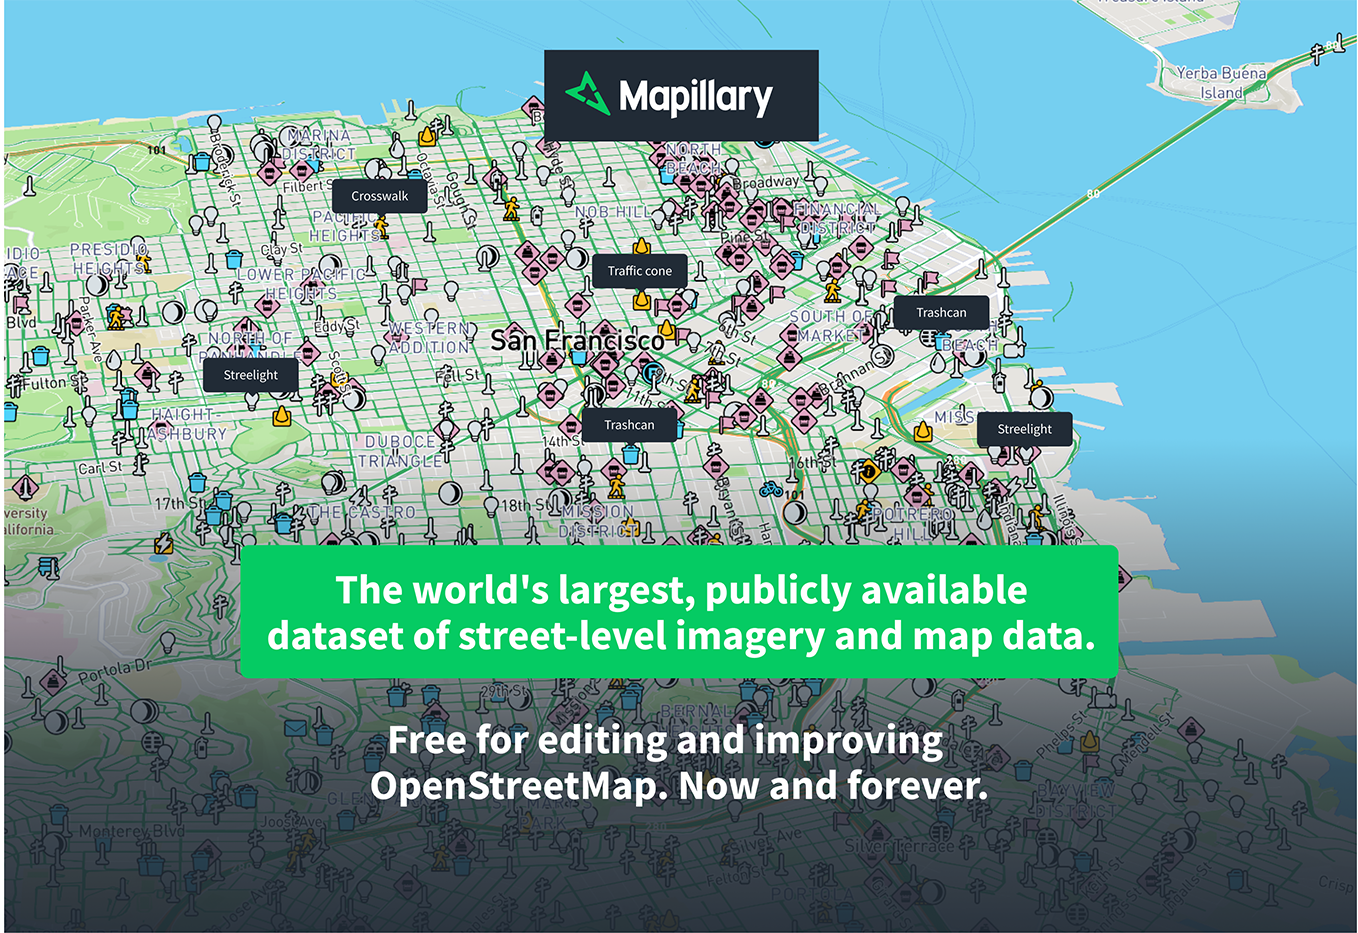
\includegraphics[width=115mm]{sponsors/mapillary.png}%
  }%
]{mapillary}
\newpairofpagestyles{sponsor-opencage-mapillary}{}
\AddLayersAtBeginOfPageStyle{sponsor-opencage-mapillary}{cropmarksevery}
\AddLayersAtBeginOfPageStyle{sponsor-opencage-mapillary}{opencage}
\AddLayersAtBeginOfPageStyle{sponsor-opencage-mapillary}{mapillary}

% IBM and OSADL advertisement
\DeclareNewLayer[background,%
  width=108mm,%
  height=77mm,%
  hoffset=8.5mm,
  voffset=7.0mm,
  contents={%
    
\includegraphics{sponsors/ibm.pdf}%
  }%
]{ibm}
\DeclareNewLayer[background,%
  width=115mm,%
  height=79mm,%
  hoffset=-0.4mm,%
  voffset=84mm,%
  contents={%
    
\includegraphics{sponsors/osadl.pdf}%
  }%
]{osadl}
\newpairofpagestyles{sponsor-ibm-osadl}{}
\AddLayersAtBeginOfPageStyle{sponsor-ibm-osadl}{ibm}
\AddLayersAtBeginOfPageStyle{sponsor-ibm-osadl}{osadl}
\AddLayersAtBeginOfPageStyle{sponsor-ibm-osadl}{cropmarksevery}

% Accenture and TomTom logo
\DeclareNewLayer[background,%
  width=84mm,%
  height=22.4mm,%
  hoffset=20mm,
  voffset=35mm,
  contents={%
    
\includegraphics[width=84mm]{sponsors/accenture.png}
  }%
]{accentureimage}
\DeclareNewLayer[background,%
  width=84mm,%
  height=25mm,%
  hoffset=18mm,
  voffset=104mm,
  contents={%
    
\includegraphics[width=97mm]{sponsors/tomtom.pdf}
  }%
]{tomtomimage}
\newpairofpagestyles[cropmarksstyle]{sponsor-accenture-tomtom}{}
\AddLayersAtBeginOfPageStyle{sponsor-accenture-tomtom}{accentureimage}
\AddLayersAtBeginOfPageStyle{sponsor-accenture-tomtom}{tomtomimage}
\AddLayersAtBeginOfPageStyle{sponsor-accenture-tomtom}{cropmarksevery}

% Facebook logo
\DeclareNewLayer[background,%
  width=83mm,%
  height=16mm,%
  hoffset=20mm,
  voffset=76mm,
  contents={%
    
\includegraphics[width=83mm]{sponsors/facebook.pdf}
  }%
]{facebookimage}
\newpairofpagestyles[cropmarksstyle]{sponsor-facebook}{}
\AddLayersAtBeginOfPageStyle{sponsor-facebook}{facebookimage}
\AddLayersAtBeginOfPageStyle{sponsor-facebook}{cropmarksevery}

% Bing logo
\DeclareNewLayer[background,%
  width=83mm,%
  height=16mm,%
  hoffset=20mm,
  voffset=67mm,
  contents={%
    
\includegraphics[width=83mm]{sponsors/bing.pdf}
  }%
]{bingimage}
\newpairofpagestyles[cropmarksstyle]{sponsor-bing}{}
\AddLayersAtEndOfPageStyle{sponsor-bing}{bingimage}
\AddLayersAtBeginOfPageStyle{sponsor-bing}{cropmarksevery}


\begin{document}
 
%\pagestyle{cropmarksstyle}
\begin{titlepage}
%  \thispagestyle{titlestyle}
  \null
\end{titlepage}
\pagestyle{cropmarksstyle}

\selectlanguage{english}
\section*{Content}
\newlength\contentspace
\setlength\contentspace{\contentspace}

\vspace*{\contentspace}%
\noindent Welcome\dotfill \pageref{welcome}
%
%\vspace*{\contentspace}%
%\noindent Scholarships \dotfill \pageref{scholarships}
%
%\vspace*{\contentspace}%
%\noindent Getting around in Milan \dotfill \pageref{getting-around}
%
%\vspace*{\contentspace}%
%\noindent Code of Conduct \dotfill \pageref{coc}

\vspace*{\contentspace}%
\noindent Saturday schedule \dotfill \pageref{saturday}

\vspace*{\contentspace}%
\noindent Social Event \dotfill \pageref{social-event}

\vspace*{\contentspace}%
\noindent Sunday schedule \dotfill \pageref{sunday}

\vspace*{\contentspace}%
\noindent Monday schedule \dotfill \pageref{monday}

\vspace*{\contentspace}%
\noindent Saturday \dotfill \pageref{saturday-descriptions}

\vspace*{\contentspace}%
\noindent Sunday \dotfill \pageref{sunday-descriptions}

\vspace*{\contentspace}%
\noindent Monday \dotfill \pageref{monday-descriptions}

\vspace*{\contentspace}%
\noindent Thanks \dotfill \pageref{thanks}

\vspace*{\contentspace}%
\noindent Sponsors \dotfill \pageref{sponsors}
%
%\vspace*{\contentspace}%
%\noindent Maps \dotfill \pageref{maps}

\vspace*{\contentspace}%
\noindent Legal notice \dotfill \pageref{legal}

\vfill
\noindent
Hashtag: \#sotm

\vspace*{0.8em}%
\noindent
The general emergency telephone number in Germany is \textbf{112}.
\vfill

\small{
\noindent
  \** Sessions in this room will not be recorded on video.\\
  \**\** This session will not be recorded on video.\\
  \diamondSymbol\ The title of this talk is not provided in full length in the schedule table. Please refer to the short description at pages \ref{abstracts}~et seqq. for the full title and list of authors.
}\normalsize


\newpage

\newpage
\enlargethispage{1\baselineskip}
\section*{Welcome to Heidelberg and State of the Map 2019} \label{welcome}
This booklet provides you essential information
about the conference, the location and the schedule.  We are proud of the participation of the
OpenStreetMap community and our rich program but there is even more!  Please do get involved and
take advantage of the off-schedule sessions, discussions and spaces.

\paragraph*{Help desk} \label{welcome-helpdesk}
You already know the help desk, located on the ground floor of the Chemie-Hörsaalgebäude (Chemistry
Lecture Halls Building). It is also your port of call if you need support or help.

\paragraph*{Programme}
You can find the diverse programme on page~\pageref{saturday}f. Full abstracts of all talks are
available at https://2019.stateofthe\\map.org/program for the general tracks and
https://2019.stateofthemap.org/academic\_programme for the academic track.

\paragraph*{Self-organised sessions} \label{welcome-location}
Rooms A, B and C in the Mathematikon building are available for self-organised sessions if they are not in use by pre-schedule sessions (see this booklet). Please come to the help desk in the Chemie-Hörsaalgebäude to announce your session.

\paragraph*{Sponsors} \label{welcome-sponsors}
We would like to thank our sponsors for making this event possible and for their support to the
OpenStreetMap Foundation.
\newpage

%\input{scholarships}
%\input{getting-around}
\newpage
\small
\renewcommand{\arraystretch}{1.4}
%\section*{Saturday Schedule}
\label{saturday}
\pagestyle{saturday-table}
\setPageBackground
\noindent\begin{landscape}
  \begin{center}
    \noindent\begin{tabular}{Z{0.75cm}Z{2.38cm};{0.2mm/2mm}Z{2.38cm};{0.2mm/2mm}Z{2.38cm};{0.2mm/2mm}Z{2.38cm};{0.2mm/2mm}}
      \cellcolor{commongray}
      &
      \multicolumn{4}{c}{
        \cellcolor{GHS}
        GHS
      }
      \tabularnewline
      \cellcolor{commongray}
      09:30
      \multiColTalk{4}{Z{9.52cm}}{Welcome}{}
      \tabularnewline
      \programHRule{5}
      \cellcolor{commongray}
      10:00
      \multiColTalk{4}{Z{9.52cm}}{\emph{Keynote} Open up! Why digital mobility needs participation}{Christian Förster, Dietmar Seifert}
      \tabularnewline
      \programHRule{5}
      \cellcolor{commongray}
      10:30
      \multiColTalk{4}{Z{9.52cm}}{\emph{Keynote}}{Karen Sandler}
      \tabularnewline
      \rowcolor{commongray}
      11:00
      & \multicolumn{4}{c}{%
      \parbox[c]{24pt}{%
        
\includegraphics[height=10pt]{cafe}%
      }
      break}
      \tabularnewline
      \cellcolor{commongray}
      & \multicolumn{1}{c}{\cellcolor{GHS} GHS}
      & \multicolumn{1}{c}{\cellcolor{HSO} HSO}
      & \multicolumn{1}{c}{\cellcolor{HSW} HSW}
      & \multicolumn{1}{c}{\cellcolor{KHS} KHS*}
      \tabularnewline
      \cellcolor{commongray}
      11:30
      \talk{Get to know OSGeo and how OSGeo is connected to OSM}{Astrid Emde}
      \talk{Data Quality and Feature Extraction at scale with RoboSat.pink}{Oliver Courtin}
      \longTalk{2}{Introduction to OSM: How it's made and how it's used}{Thomas Skowron, Frederik Ramm}
      \longTalk{2}{\emph{Workshop}\linebreak Mapping public transport and cycling itineraries using JOSM's PT\_Assistant plugin}{Polyglot}
      \tabularnewline
      \programCRule{2-3}
      \cellcolor{commongray}
      12:00
      \talk{``Keepin' it fresh (and good)!''\,\diamondSymbol}{Kevin Ventullo, Christopher Klaiber}
      \talk{Human Mapping with Machine Data}{Christopher Beddow, Edoardo Neerhut}
      &
      &
      \tabularnewline
      \programCRule{2-3}
      \programCRule{5-5}
    \end{tabular}
    \newpage

    \noindent\begin{tabular}{Z{0.75cm}Z{2.38cm};{0.2mm/2mm}Z{2.38cm};{0.2mm/2mm}Z{2.38cm};{0.2mm/2mm}Z{2.38cm};{0.2mm/2mm}}
      \cellcolor{commongray}
      & \multicolumn{1}{c}{\cellcolor{GHS} GHS}
      & \multicolumn{1}{c}{\cellcolor{HSO} HSO}
      & \multicolumn{1}{c}{\cellcolor{HSW} HSW}
      & \multicolumn{1}{c}{\cellcolor{KHS} KHS*}
      \tabularnewline
      \cellcolor{commongray}
      12:30
      \talk{Driving South East Asia Forward with OpenStreetMap}{Jinal Foflia}
      \talk{Assisted Intelligence~-- How we map with the support of new technologies}{Felix Delattre, Surabhi Singh}
      &
      &
      \tabularnewline
      \rowcolor{commongray}
      13:00
      & \multicolumn{4}{c}{%
      \parbox[c]{24pt}{%
        
\includegraphics[height=10pt]{restaurant}%
      }
      lunch}
      \tabularnewline
      \cellcolor{commongray}
      14:00
      \talk{ODbL license compatibility}{Kathleen Lu}
      \talk{Lightning Talks I}{}
      \longTalk{2}{Share Edits and Insights with the Overpass Tools}{Roland Olbricht}
      \longTalk{2}{\emph{Workshop}\linebreak How to contribute to weeklyOSM via the CMS: OSMBC}{Manfred Reiter}
      \tabularnewline
      \programCRule{2-3}
      \cellcolor{commongray}
      14:30
      \talk{Communication and Knowledge Transfer in OSM}{Hanna Krüger}
      \talk{OsmInEdit~-- a simple indoor editor}{Adrien Pavie et\,al.}
      &
      &
      \tabularnewline
      \programHRule{5}
      \cellcolor{commongray}
      15:00
      \talk{Past and Future of the OSMF Membership Working Group}{Michael Spreng}
      \talk{Observe~-- offline, cross-platform field mapping tool for OpenStreetMap}{Sajjad Anwar}
      &
      &
      \tabularnewline
      \programHRule{5}
    \end{tabular}
    \newpage

    \noindent\begin{tabular}{Z{0.75cm}Z{2.38cm};{0.2mm/2mm}Z{2.38cm};{0.2mm/2mm}Z{2.38cm};{0.2mm/2mm}Z{2.38cm};{0.2mm/2mm}}
      \cellcolor{commongray}
      & \multicolumn{1}{c}{\cellcolor{GHS} GHS}
      & \multicolumn{1}{c}{\cellcolor{HSO} HSO}
      & \multicolumn{1}{c}{\cellcolor{HSW} HSW}
      & \multicolumn{1}{c}{\cellcolor{KHS} KHS*}
      \tabularnewline
      \rowcolor{commongray}
      15:30
      & \multicolumn{4}{c}{%
      \parbox[c]{24pt}{%
        
\includegraphics[height=10pt]{photo}%
      }
      photo (courtyard of Mathematikon building)}
      \tabularnewline
      \rowcolor{commongray}
      16:00
      & \multicolumn{4}{c}{%
        \parbox[c]{24pt}{%
          
\includegraphics[height=10pt]{cafe}%
        }
      break}
      \tabularnewline
      \cellcolor{commongray}
      16:30
      \talk{OSM Data: From Digital to Physical Design}{Yantisa Akhadi}
      \talk{Lightning Talks II}{}
      \longTalk{2}{Board and working groups meeting \emph{(public)}}{}
      \longTalk{2}{\emph{Workshop}\linebreak uMap for newbies}{Manfred Reiter}
      \tabularnewline
      \programCRule{2-3}
      \cellcolor{commongray}
      17:00
      \talk{CyclOSM, a bicycle oriented render for every cyclist}{Lucas Verney, Florimond Berthoux}
      \talk{VR Map: Using OSM Data In a WebVR Environment}{Robert Kaiser}
      &
      &
      \tabularnewline
      \programCRule{2-3}
      \programCRule{5-5}
      \cellcolor{commongray}
      17:30
      \talk{How to use OSM data with the Desktop GIS QGIS}{Astrid Emde}
      \talk{Hikar~-- OSM Augmented Reality for Walkers across Europe}{Nick Whitelegg}
      &
      &
      \tabularnewline
      \programHRule{5}
    \end{tabular}
    \newpage

    \label{social-event}%
    \enlargethispage{1\baselineskip}%
    \newlength\socialEventBoxWidth
    \setlength{\socialEventBoxWidth}{10.82cm}
    \newlength\socialEventSectionSep
    \setlength{\socialEventSectionSep}{\baselineskip}
    \noindent\begin{tabular}{Z{0.75cm}Z{\socialEventBoxWidth};{0.2mm/2mm}}
      \rowcolor{ochsenblutrot}
      \parbox[t]{\linewidth}{%
        \textcolor{white}{19:00}%
      }%
      &
      \multicolumn{1}{C{\socialEventBoxWidth}}{%
        \textcolor{white}{%
          Social Event at Hebelhalle
        }%
      }
      \tabularnewline
      \cellcolor{ochsenblutrot}
      &
      \begin{minipage}[t]{\socialEventBoxWidth}
        \noindent\begin{minipage}[t]{0.47\linewidth}
          \vspace{-0.56\baselineskip}
          \begin{wrapfigure}[6]{r}[0pt]{0.4\linewidth}%
            \vspace{-1\baselineskip}%
            \qrcode[height=18mm,padding]{geo:49.39655,8.67945}%
          \end{wrapfigure}%
          \textbf{Location}\\
          Hebelhalle\\
          Hebelstraße 9\\
          69115 Heidelberg\\
          geo:49.39655,8.67945\\
          entrance from Gottlieb-Daimler-Straße

          \vspace{\socialEventSectionSep}
          \textbf{Getting there by public transport}\\
          next tram stop: Rudolf-Diesel-Straße\\
          tram line 26, bus line 33

          \vspace{\socialEventSectionSep}
          \textbf{Programme}\\
          Welcome\\
          Dinner and music\\
          OSM Awards ceremony

          \vspace{\baselineskip}
          Catering is provide by a local catering company employing refugees from Syria.
        \end{minipage}
        \hfill
        \noindent\begin{minipage}[t]{0.47\linewidth}
          \begin{center}
            \noindent tabbouleh salad with fried shrimps\\
            $\blackdiamond$\\
            couscous salad with fried vegetables and herbs\\
            $\blackdiamond$\\
            baguette with hummus and sprouts and dried tomatoes\\
            $\blackdiamond$\\
            fresh figs and prickly pears with balsamic reduction, soft goats cheese, ham and bread\\
            $\blackdiamond$\\
            stewed beef in orange, cocos and fresh coriander sauce, rice\\
            $\blackdiamond$\\
            Syrian dal from lentils with lime, spices, fresh herbs, cocos milk and pumpkin topping, rice\\
            $\blackdiamond$\\
            desserts

            \noindent \emph{The menu might be subject of change.}
          \end{center}
        \end{minipage}
      \end{minipage}
      \vspace{0.4\multicolsep}
      \tabularnewline
      \programHRule{2}
    \end{tabular}
  \end{center}
  \newpage
\end{landscape}
\renewcommand{\arraystretch}{1.0}

\newpage
\renewcommand{\arraystretch}{1.4}
%\section*{Sunday Schedule}
\label{sunday}
\pagestyle{sunday-table}
\setPageBackground
\noindent\begin{landscape}
  \begin{center}
    \enlargethispage{1\baselineskip}
    \noindent\begin{tabular}{Z{0.75cm}Z{2.18cm}|Z{2.38cm}|Z{3.26cm}|Z{1.7cm}|}
      \cellcolor{table-header}
      &
      \multicolumn{4}{c}{
        \tableColHead{Hörsaal West}
      }
      \tabularnewline
      \cellcolor{table-header}
      09:00
      &
      \multicolumn{4}{Z{9.7cm}|}{%
        \textbf{Bridging the Map? Exploring Interactions between the Academic and Mapping Communities in OSM}
        % no newline to save space
        \hspace{1em}
        \emph{A. Yair Grinberger et\,al.}%
      }
      \tabularnewline
      \cellcolor{table-header}
      & \multicolumn{1}{c}{\tableColHead{Großer Hörsaal}}
      & \multicolumn{1}{c}{\tableColHead{Hörsaal Ost}}
      & \multicolumn{1}{c}{\tableColHead{Hörsaal West}}
      & \multicolumn{1}{c}{\tableColHead{KHS~\noVideo}}
      \tabularnewline
      \tableRowFirstCell{09:30}
      \talk{Flexible Routing with Graph\-Hopper}{Peter Karich}
      \talk{``Mapathon, Mapathon, Mapathon!''}{Séverin Menard, Nicolas Chavent}
      \talk{OpenStreetMap as a Space~\noVideo}{Dipto Sarkar, So Hoi Kay}
      \longTalk{3}{Scholar\linebreak Lightning\linebreak Talks}{}
      \tabularnewline
      \programHRule{4}
      \tableRowFirstCell{10:00}
      \talk{Imagery\linebreak Solutions in OSM}{Kevin Bullock}
      \talk{Associations Dynamics in French Speaking Africa\,\diamondSymbol}{Séverin Menard, Nicolas Chavent}
      \talk{Analysis of OSM Data through OSM Notes User Posting}{Toshikazu Seto et\,al.}
      &
      \tabularnewline
      \programHRule{4}
      \tableRowFirstCell{10:30}
      \talk{Lightning\linebreak Talks III}{}
      \talk{Tales from the Tasking Manager}{Ramya Ragupathy et\,al.}
      \talkSingleLine{A Novel Application of Models of Species Abundance to Better Understand OSM Community Structure and Interactions}{P. Mooney}
      &
      \tabularnewline
      \programHRule{5}
    \end{tabular}
  \end{center}
  \newpage

  \begin{center}
    \noindent\begin{tabular}{Z{0.75cm}Z{1.80cm}|Z{1.80cm}|Z{2.60cm}|Z{1.40cm}|Z{1.50cm}|}
      \cellcolor{table-header}
      & \multicolumn{1}{c}{\tableColHead{Großer Hörsaal}}
      & \multicolumn{1}{c}{\tableColHead{Hörsaal Ost}}
      & \multicolumn{1}{c}{\tableColHead{Hörsaal West}}
      & \multicolumn{1}{c}{\tableColHead{KHS~\noVideo}}
      & \multicolumn{1}{c}{\tableColHead{Math. C~\noVideo}}
      \tabularnewline
      \tableRowFirstCell{11:00}
      &
      \multicolumn{5}{c}{%
        \cellcolor{commongray}
        \parbox[c]{24pt}{%
          
\includegraphics[height=10pt]{cafe}%
        }%
        Break%
      }
      \tabularnewline
      \tableRowFirstCell{11:30}
      \talk{Overview of Map Serving Architectures}{Paul Norman}
      \talk{Our Falkirk~-- Mitigating the Impacts of Poverty\,\diamondSymbol}{Alison Moon}
      \talk{Towards Scalable Geospatial Remote Sensing for Efficient OSM Labeling\,~\noVideo}{Rui Zhang et\,al.}
      \longTalk{3}{Bilingual Breakout Session}{Séverin Menard, Nicolas Chavent}
      \longTalk{2}{\emph{Workshop}\linebreak First steps with OSM\linebreak Editors}{Angjelina Dervishaj}
      \tabularnewline
      \programCRule{2-4}
      \tableRowFirstCell{12:00}
      \talk{Customising Search for Special-Interest Maps}{S. Hoffmann}
      \talk{Metrics to Monitor\linebreak Buildings\linebreak Outbounds\,\diamondSymbol}{Pierre Béland}
      \talk{Estimating Latent Energy Demand of Buildings}{Nikola Milojevic-Dupont et\,al.}
      &
      &
      \tabularnewline
      \programCRule{2-4}
      \programCRule{6-6}
      \tableRowFirstCell{12:30}
      \talk{Is Your OSM App Spying on You?}{Thomas Skowron}
      \talk{Integrating Quality Assurance Checks into Map \mbox{Editors}\,\diamondSymbol}{David Manzer et\,al.}
      \talk{Client-Side Route Planning: Preprocessing the OSM Road Network for Routable Tiles}{Harm Delva et\,al.}
      &
      &
      \tabularnewline
      \programHRule{6}
    \end{tabular}
  \end{center}
  \newpage

  \begin{center}
    \noindent\begin{tabular}{Z{0.75cm}Z{2.00cm}|Z{1.80cm}|Z{2.30cm}|Z{1.50cm}|Z{1.60cm}|}
      \cellcolor{table-header}
      & \multicolumn{1}{c}{\tableColHead{Großer Hörsaal}}
      & \multicolumn{1}{c}{\tableColHead{Hörsaal Ost}}
      & \multicolumn{1}{c}{\tableColHead{Hörsaal West}}
      & \multicolumn{1}{c}{\tableColHead{KHS~\noVideo}}
      & \multicolumn{1}{c}{\tableColHead{Math. C~\noVideo}}
      \tabularnewline
      \rowcolor{commongray}
      \tableRowFirstCell{13:00}
      &
      \multicolumn{5}{c}{%
        \cellcolor{commongray}
        \parbox[c]{24pt}{%
          
\includegraphics[height=10pt]{restaurant}%
        }%
        Lunch%
      }
      \tabularnewline
      \tableRowFirstCell{14:00}
      \talk{What's behind JOSM?}{Vincent Privat}
      \talk{Spatial Indexes for OSM in PostGIS}{Felix Kunde}
      \talk{Intrinsic Assessment of Contri\-bution Patterns through Explora\-tory Spatial Data Analysis}{Marco Minghini et\,al.}
      \longTalk{2}{Diversity and Inclusion in OSM}{Patricia Solis et\,al.}
      \longTalk{2}{\emph{Workshop}\linebreak Using \mbox{OSMCha} to Understand Bad Edits}{Andrey Golovin et\,al.}
      \tabularnewline
      \programCRule{2-4}
      \tableRowFirstCell{14:30}
      \talk{Mapping Solar Panels Can Save Megatons of CO\textsubscript{2}}{Dan Stowell, Jerry Clough}
      \talk{Lightning Talks IV}{}
      \talk{Corporate Editors in the Evolving Landscape of OSM: A Close Investigation of the Impact to the Map and Community}{Jennings Anderson et\,al.}
      &
      &
      \tabularnewline
      \programHRule{6}
    \end{tabular}
  \end{center}
  \newpage

  \begin{center}
    \noindent\begin{tabular}{Z{0.75cm}Z{2.00cm}|Z{1.80cm}|Z{2.30cm}|Z{1.50cm}|Z{1.60cm}|}
      \cellcolor{table-header}
      & \multicolumn{1}{c}{\tableColHead{Großer Hörsaal}}
      & \multicolumn{1}{c}{\tableColHead{Hörsaal Ost}}
      & \multicolumn{1}{c}{\tableColHead{Hörsaal West}}
      & \multicolumn{1}{c}{\tableColHead{KHS~\noVideo}}
      & \multicolumn{1}{c}{\tableColHead{Math. C~\noVideo}}
      \tabularnewline
      \tableRowFirstCell{15:00}
      \talk{National Trust~-- Managing a Path Inventory in OSM: Towards an Open Paths Standard in OSM for the UK}{Huw Davies}
      \longTalk{2}{OSM Data Processing with PostgreSQL/\allowbreak PostGIS}{Jochen Topf}
      \talk{Exploring the \mbox{Effects} of Pokémon Go Vandalism on OSM}{Levente Juhász et\,al.}
      \longTalk{2}{Nomad Maps, an Andean Cartographic Itinerancy by Bike \emph{(Video)}}{Alban Vivert}
      \bookableSpace
      \tabularnewline
      \programCRule{2-2}
      \programCRule{4-4}
      \programCRule{6-6}
      \tableRowFirstCell{15:30}
      \talk{Collaborative Mapping of Cycling Infrastructure for Route and Thematic Maps~\diamondSymbol}{Carolina Ortega Espinosa}
      &
      \talk{Analysing the Spatio-Temporal Patterns and Impacts of Large-Scale Data Production Events in OSM}{A. Yair Grinberger et\,al.}
      &
      \bookableSpace
      \tabularnewline
      \tableRowFirstCell{16:00}
      &
      \multicolumn{5}{c}{%
        \cellcolor{commongray}
        \parbox[c]{24pt}{%
          
\includegraphics[height=10pt]{cafe}%
        }%
        Break%
      }
      \tabularnewline
    \end{tabular}
  \end{center}
  \newpage

  \begin{center}
    \noindent\begin{tabular}{Z{0.75cm}Z{2.20cm}|Z{1.30cm}|Z{2.70cm}|Z{1.40cm}|Z{1.60cm}|}
      \cellcolor{table-header}
      & \multicolumn{1}{c}{\tableColHead{Großer Hörsaal}}
      & \multicolumn{1}{c}{\tableColHead{Hörsaal Ost}}
      & \multicolumn{1}{c}{\tableColHead{Hörsaal West}}
      & \multicolumn{1}{c}{\tableColHead{KHS~\noVideo}}
      & \multicolumn{1}{c}{\tableColHead{Math. C~\noVideo}}
      \tabularnewline
      \tableRowFirstCell{16:30}
      \talk{Notes: Can We Do Better.\linebreak Experiences and Ideas from the Frontline}{Chris Fleming}
      \talk{Mapper's Privacy}{Roland Olbricht}
      \talk{Development after Displacement: Using OSM Data to Measure SDG Indicators at Informal Settlements}{Hannah Friedrich et\,al.}
      \talk{Updating our Attribution Guidelines}{Simon Poole}
      \longTalk{2}{\emph{Workshop}\linebreak JOSM Turn Restriction: Improving Data Quality}{Harry Mahardhika Machmud}
      \tabularnewline
      \programCRule{2-5}
      \tableRowFirstCell{17:00}
      \talk{Is the OSM Data Model Creaking?}{Martin Lucas-Smith}
      \talk{Teams for OSM}{Marc Farra}
      \talk{Analysis of OSM Data Quality at Different Stages of a Participatory Mapping Process: Evidence from Informal Urban Settings}{Godwin Yeboah et\,al.}
      \longTalk{2}{Local Chapters Congress}{Joost Schouppe}
      &
      \tabularnewline
      \programCRule{2-4}
      \programCRule{6-6}
      \tableRowFirstCell{17:30}
      \talk{Broken Promises and Technical Difficulties}{Ilya Zverv}
      \talk{Lightning Talks V}{}
      \talk{Assessing the Completeness of Urban Green Spaces in OSM}{Christina Ludwig et\,al.}
      &
      &
      \tabularnewline
      \programHRule{6}
    \end{tabular}
    \newpage

    \label{poster-event}%
    \setlength{\socialEventBoxWidth}{10.82cm}
    \setlength{\socialEventSectionSep}{\baselineskip}
    \noindent\begin{tabular}{Z{0.75cm}Z{\socialEventBoxWidth}|}
      \rowcolor{ochsenblutrot}
      \parbox[t]{\linewidth}{%
        \textcolor{white}{18:00}%
      }%
      &
      \multicolumn{1}{C{\socialEventBoxWidth}}{%
        \textcolor{white}{%
          Poster Session at Mathematikon
        }%
      }
      \tabularnewline
      \cellcolor{ochsenblutrot}
      &
      \begin{minipage}[t]{\socialEventBoxWidth}
        \vspace{0.2\baselineskip}
        \noindent\begin{minipage}[c]{0.4\linewidth}
          \RaggedRight
          We invite you to join the poster session with the exhibition
          of posters accepted by the academic programme committee and
          the submissions of the open poster competition.

          Drinks, some food and our special State of the Map 2019 beer will be provided.

          \vspace{\socialEventSectionSep}
          \textbf{Location}\\
          Mathematikon\\
          Klaus-Tschira-Platz\\
          69120 Heidelberg\\
          geo:49.4172,8.6755\\
          entrance from the south, ground floor 
          \justifying
        \end{minipage}
        \hfill
        \noindent\begin{minipage}[c]{0.57\linewidth}
          \begin{center}
            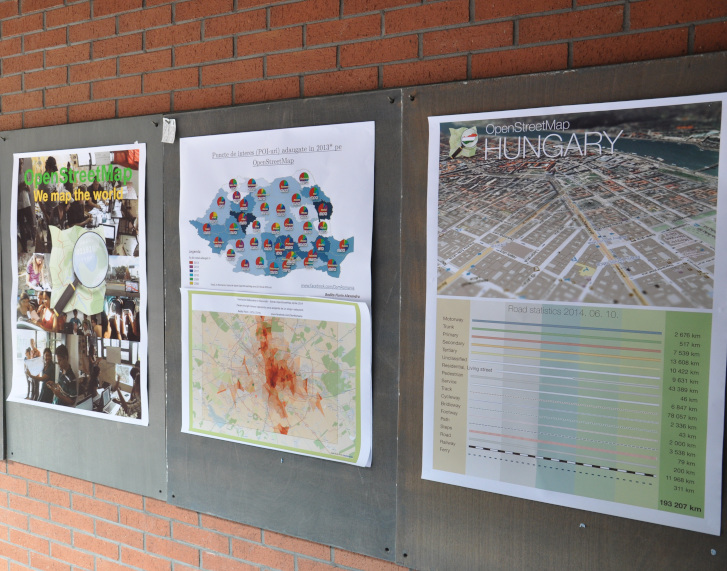
\includegraphics[width=0.9\linewidth]{images-print/posters-sotm-eu-2014.jpg}

            \qrcode[height=18mm,padding]{geo:49.41722,8.67550}%
          \end{center}
        \end{minipage}
      \end{minipage}
      \vspace{0.4\multicolsep}
      \tabularnewline
      \programHRule{2}
    \end{tabular}
  \end{center}
\end{landscape}
\renewcommand{\arraystretch}{1.0}
\normalsize

%\newpage
\small
\renewcommand{\arraystretch}{1.4}
%\section*{Monday Schedule}
\label{monday}
\pagestyle{monday-table}
\setPageBackground
\noindent\begin{landscape}
  \begin{center}
    \noindent\begin{tabular}{Z{0.75cm}Z{2.38cm}|Z{2.38cm}|Z{2.38cm}|Z{2.38cm}|}
      \cellcolor{commongray}
      & \multicolumn{1}{c}{\cellcolor{GHS} Großer Hörsaal}
      & \multicolumn{1}{c}{\cellcolor{HSO} Hörsaal Ost}
      & \multicolumn{1}{c}{\cellcolor{KHS} Kleiner Hörsaal~\noVideo}
      & \multicolumn{1}{c}{\cellcolor{Mathematikon C} Mathematikon C~\noVideo}
      \tabularnewline
      \cellcolor{commongray}
      09:30
      \talk{Qwant Maps: Geocode the World with OSM Data}{Guillaume et\,al.}
      \talk{OSM2World: 3D OSM in Your Browser}{Tobias Knerr}
      \longTalk{2}{The Next Generation of Mappers: Learning from YouthMappers}{Jessica Bergmann}
      \longTalk{2}{\emph{Workshop}\linebreak OpenStreetMap and Wikidata: Awesome Together}{Eugene Alvin Villar}
      \tabularnewline
      \programCRule{2-3}
      \cellcolor{commongray}
      10:00
      \talk{Routing for \mbox{Humans}}{Sebastian Ritterbusch}
      \talk{OpenDatathon Activities in Japan}{Shinji Enoki}
      &
      &
      \tabularnewline
      \programHRule{5}
      \cellcolor{commongray}
      10:30
      \talk{Mapping Mobility in Stockport}{Sam Milson}
      \talk{Lightning Talks IV}{}
      \talk{OpenStreetMap in Croatia}{Hrvoje Bogner}
      &
      \tabularnewline
      \rowcolor{commongray}
      11:00
      & \multicolumn{4}{c}{%
      \parbox[c]{24pt}{%
        
\includegraphics[height=10pt]{cafe}%
      }
      Break}
    \end{tabular}

    \noindent\begin{tabular}{Z{0.75cm}Z{2.38cm}|Z{2.38cm}|Z{2.38cm}|Z{2.38cm}|}
      \cellcolor{commongray}
      & \multicolumn{1}{c}{\cellcolor{GHS} Großer Hörsaal}
      & \multicolumn{1}{c}{\cellcolor{HSO} Hörsaal Ost}
      & \multicolumn{1}{c}{\cellcolor{KHS} Kleiner Hörsaal~\noVideo}
      & \multicolumn{1}{c}{\cellcolor{Mathematikon C} Mathematikon C~\noVideo}
      \tabularnewline
      \cellcolor{commongray}
      11:30
      \longTalk{2}{Caretography~-- Mapping Difficult Issues with OpenStreetMap during Difficult Times}{David Garcia, Martin Dittus}
      \talk{Integrating and Validating Open Data in OSM Using Street Pictures}{Andrien Pavie}
      \longTalk{2}{New processes to Agree on Tagging Suggestions and Their Interaction with the Editing Software Available on osm.org}{Roland Olbricht}
      \longTalk{2}{\emph{Workshop}\linebreak Custom Presets Creation Using JOSM}{Harry Mahardhika Machmud}
      \tabularnewline
      \programCRule{3-3}
      \cellcolor{commongray}
      12:00
      &
      \talk{Introduce OpenPlaceReviews and Connect to OSM}{Victor Shcherb}
      &
      &
      \tabularnewline
      \programHRule{5}
      \cellcolor{commongray}
      12:30
      \talk{Access to\linebreak Prosperity: Quantifying Infrastructure Impact with OSM}{Davey Lovin}
      \talk{Lightning Talks VII}{}
      &
      &
      \tabularnewline
      \rowcolor{commongray}
      13:00
      & \multicolumn{4}{c}{%
        \parbox[c]{24pt}{%
          
\includegraphics[height=10pt]{restaurant}%
        }
      Lunch}
    \end{tabular}

    \noindent\begin{tabular}{Z{0.75cm}Z{2.38cm}|Z{2.38cm}|Z{2.38cm}|Z{2.38cm}|}
      \cellcolor{commongray}
      & \multicolumn{1}{c}{\cellcolor{GHS} Großer Hörsaal}
      & \multicolumn{1}{c}{\cellcolor{HSO} Hörsaal Ost}
      & \multicolumn{1}{c}{\cellcolor{KHS} Kleiner Hörsaal~\noVideo}
      & \multicolumn{1}{c}{\cellcolor{Mathematikon C} Mathematikon C~\noVideo}
      \tabularnewline
      \cellcolor{commongray}
      14:00
      \talk{Pedestrian Routing in Complex Areas: the Case of Paris Railway Stations}{Antoine Riche}
      \talk{Norway: Successful Deployment of OSM in Public Transport}{Johan Wiklund}
      \talk{Participatory Mapping for Open Counties}{Zacharia Muindi}
      \longTalk{2}{\emph{Workshop}\linebreak ImproveOSM~-- MissingRoads Workshop}{Beata Tautan-Jancso, Dumitru Laura}
      \tabularnewline
      \programCRule{2-4}
      \cellcolor{commongray}
      14:30
      \talk{Automatically\linebreak Annotate a Pedestrian Route with OSM Landmarks}{Frédéric Rodrigo}
      \talk{Public Transport Navigation Using OSM by OsmAnd}{Victor Shcherb, Eugene Kizevich}
      &
      &
      \tabularnewline
      \programHRule{5}
      \cellcolor{commongray}
      15:00
      \talk{From Car Routing to Train Routing~\noVideo}{Denis Cheynet}
      \talk{OSM Vector Tiles in Custom Coordinate Systems}{Jiri Komarek}
      \talk{State of the Map Bangladesh: Transforming a Resilient Community by Institutionalising~\diamondSymbol}{Tasauf A Baki Billah}
      &
      \tabularnewline
      \rowcolor{commongray}
      15:30
      & \multicolumn{4}{c}{%
      \parbox[c]{24pt}{%
        
\includegraphics[height=10pt]{cafe}%
      }
      Break}
      \tabularnewline
      \cellcolor{commongray}
      16:00
      \talk{Closing}{}
      &
      &
      &
      \tabularnewline
      \programHRule{5}
    \end{tabular}
  \end{center}
  \renewcommand{\arraystretch}{1.0}

  \newpage
  \pagestyle{cropmarksstyle}
  \sponsorBoxLandscape{%
    images-print/osmf-banner.png%
  }{%
    40mm
  }{%
    4
  }{%
    The OpenStreetMap Foundation is the 
    international non-profit organisation
    supporting, but not controlling,
    OpenStreetMap. We are dedicated to
    encouraging the growth, development and
    distribution of free geospatial data and to
    providing geospatial data for anyone to use
    and share.
    
    We need you as member. Members are vital
    to the OpenStreetMap Foundation---to voice ideas
    and shape the direction of the Foundation,
    and support efforts of working groups. We
    welcome all who support our goals to join us!
    
    Find out more and join at osmfoundation.org
    or join our sessions:
    \begin{itemize}
      \RaggedRight
      \setlength{\itemsep}{-3pt} % Aufzählungspunktabstand auf 0
      \item Saturday 14:00, Großer Hörsaal: ODbL licence compatiblity
      \item Saturday 15:00, Großer Hörsaal: Past and Future of the OSMF Membership Working Group
      \item Saturday 16:30, Hörsaal West: Board and working groups meeting
      \item Sunday 16:30, Kleiner Hörsaal: Updating our attribution guidelines
      \item Sunday 17:00, Kleiner Hörsaal: Local chapter congress
    \end{itemize}
    \justifying
  }%


  \setlength{\fboxsep}{4.5pt}%
  \vspace{0.5\baselineskip}%
  \noindent%
  \fcolorbox{gray}{white}{%
    \parbox{\fboxwidth}{%
      \parbox{0.82\fboxwidth}{%
        \noindent Video recording and streaming is provided
        by the volunteers of CCC Video Operation Centre.
        The videos will be published at https://media.ccc.de/ under
        a free and open licence.
      }%
      \hfill%
      \parbox{0.15\fboxwidth}{%
        \begin{center}
          
\includegraphics[width=12mm]{images-print/voc.pdf}%
        \end{center}
      }%
    }%
  }
  \setlength{\fboxsep}{3pt}

\end{landscape}

\newpage

%\input{lightning-talks}
%\input{osmf}
%\newpage
\section*{Thanks}
\label{thanks}
\pagestyle{cropmarksstyle}
%% short version:
% This conference would not have been possible with the huge support by a lot of volunteers. We would like to thank

Each year when we write this section we are reminded why OpenStreetMap is so great---it's the dedication
and passion of individuals who, when acting together, can achieve great things. This year is no
different. In fact we've been helped by a record number of people, many of whom are returning in
roles they supported in the previous year or two. The generosity of the following people have kept
us on track and each contribution, however small, moved us closer to our goal. Thank you.

\newlength{\volunteerSpace}
\setlength\volunteerSpace{0.8\baselineskip}
\RaggedRight
\begin{multicols}{2}
  \begin{small}
    \textbf{SotM Working Group}\\
    Benoît Fournier\\
    Christine Karch\\
    Gregory Marler\\
    Marco Minghini\\
    Michael Reichert\\
    Mikel Maron\\
    Rob Nickerson

    \vspace{\volunteerSpace}
    \textbf{Local team}\\
    Adam Rousell\\
    Christina Ludwig\\
    Fabian Kowatsch\\
    Martin Raifer\\
    Melanie Eckler\\
    Rafael Troilo\\
    Sven Lautenbach\\

    \vspace{\volunteerSpace}
    \textbf{Academic selection committee}\\
    A. Yair Grinberger\\
    Godwin Yeboah\\
    Levente Juhász\\
    Marco Minghini\\
    Peter Mooney

    \vspace{\volunteerSpace}
    \textbf{Programme selection \mbox{committee}}\\
    Astrid Emde\\
    Benoît Fournier\\
    Christine Karch\\
    Gregory Marler\\
    Ilya Zverev\\
    Jennings Anderson\\
    Manfred Stock\\
    Martin Raifer\\
    Mats'eliso Thobei\\
    Nelson A. de Oliveira\\
    Sarah Hoffmann\\
    Satoshi Iida\\
    Sidorela Uku\\
    Séverin Menard

    \vspace{\volunteerSpace}
    \textbf{Scholarship selection}\\
    %TODO Is this list correct?
    Arnalie Faye Vicario\\
    Geoffrey Kateregga\\
    Kshitiz Khanal\\
    Laura Mugeha\\
    Michael Reichert\\
    Montseng Moeti\\
    Rebecca Firth\\
    Remígio Chilaule\\
    Samaila Alio Mainassara\\
    Sebastian Meier\\
    Sven Lautenbach\\
    Timofey Subbotin\\
    Yiming Zhu\\

    \vspace{\volunteerSpace}
    \textbf{Video recording}\\
    saerdner\\
    MichaelK\\
    mgehling\\
    Nakaner\\
    NHG

    \vspace{\volunteerSpace}
    \textbf{Other}\\
    Dorothea Kazazi (scholarship and admin support)\\
    Frederik Ramm (treasurer)\\
    Ilya Zverev (OSM Awards lead)\\
    Manfred Reiter (volunteer management)\\
    Tom Hughes (ticket site)\\
  \end{small}
\end{multicols}

\section*{Sponsors}
\label{sponsors}
%TODO If space permits, add this section, otherwise remove it.
\RaggedRight
\begin{multicols}{2}
  \begin{small}
    \textbf{Platinum}\\
    Ministry of Transport Baden-Württemberg\\

    \vspace{\volunteerSpace}
    \textbf{Gold}\\
    Bing/Microsoft\\
    Facebook\\
    Mapbox\\

    \vspace{\volunteerSpace}
    \textbf{Silver}\\
    Anyways\\
    Geotab\\
    Grab\\
    Telenav\\
    TomTom\\

    \vspace{\volunteerSpace}
    \textbf{Bronze}\\
    Accenture\\
    IBM\\
    Mapillary\\
    Maxar\\
    OSADL\\
    OpenCage\\
    SNCF\\

    \vspace{\volunteerSpace}
    \textbf{Supporters}\\
    Bergfex\\
    Disy\\
    Geofabrik\\
    Omniscale\\
    Sinergise\\
    WhereGroup\\
    YellowMap\\

  \end{small}
\end{multicols}

\justifying

\newpage
\pagestyle{cropmarksstyle}
\noindent
\vspace{10mm}
\begin{center}
  
\includegraphics[width=0.8\linewidth]{sponsors/accenture.png}
\end{center}
\newpage
\null
\newpage

\section*{Legal Notice and Credits}
\label{legal}

\RaggedRight
State of the Map 2019 is jointly organised by the OpenStreetMap Foundation,
Ruprecht-Karls-Universität Heidelberg and FOSSGIS e.V..

\vspace{0.5em}
\newlength\logoHeight
\setlength{\logoHeight}{3.5\baselineskip}

\includegraphics[height=\logoHeight]{osm-logo.pdf}
\hfill

\includegraphics[height=\logoHeight]{uni_hd_logo.pdf}
\hfill

\includegraphics[height=0.8\logoHeight]{FOSSGIS.pdf}

\vspace{0.5em}
\noindent Responsible for the content:\\
OpenStreetMap Foundation\\
St John’s Innovation Centre\\
Cowley Road\\
Cambridge\\
CB4 0WS\\
United Kingdom

\vspace{0.5em}
\noindent This booklet has been prepared using Lua\LaTeX\ and 
other free and open-source software.\\
Source code: https://github.com/osmfoundation/sotm2019-booklet\\
Content: State of the Map Working Group\\
Copy editing: Jez Nicholson, Michael Booth, Christine Karch, Rory McCann\\
Typesetting and layout: Michael Reichert, Martin Raifer\\
Map style and icons in the schedules: OpenStreetMap Carto developers\\
Map data: 
\includegraphics[height=7pt]{copyright}~Open\-Street\-Map contributors, published unter Open Database License, see https://osm.org/copyright for more information\\
OpenStreetMap logo: Ken Vermette, CC-BY-SA~2.0

\vspace{1em}
\noindent \begin{minipage}[htbp]{0.2\textwidth}
\noindent
\includegraphics[width=\linewidth]{cc-by-sa-pdf}
\end{minipage}
\hfill
\begin{minipage}[hbtp]{0.74\textwidth}\RaggedRight
  {\small
    This booklet may be re-used under the Creative Commons Attribution Share-Alike 3.0 license.
    This does not apply to advertisements and logos.
  }
\end{minipage}
\newpage

\pagestyle{page-public-transport}
\label{public-transport-map}
\null
\newpage
\pagestyle{page-citymap-left}
\label{maps}
\null
\newpage
\pagestyle{page-citymap-right}
\null
\newpage
\pagestyle{page-campus}
\null

%\input{back_cover}

\end{document}
